\section{\datasetname}
\label{saas}

\subsection{SaaS 环境}
\label{saas-env}

\datasetname 建立在真实、开源且可部署的 SaaS 系统之上，而非玩具网站或静态网页。图~\ref{fig:eval} 展示了 \datasetname 的整体框架。我们依据三项标准选取 23 个 SaaS 系统。第一，每个系统都应是具有完整前后端逻辑、用户认证、持久化数据库状态和领域业务约束的真实软件应用，以提供接近生产环境的交互复杂度。第二，所选系统应覆盖广泛的专业场景，使任务设计能够涉及多种职业角色。第三，我们优先选择适合构建跨应用工作流的系统，使功能互补的应用能够自然组合为多系统任务，而非彼此隔离的单网站操作。

为支持专业任务构建，我们把这 23 个 SaaS 系统划分到六个领域：软件工程与项目管理（\textbf{Software.}）、业务运营与财务（\textbf{Business.}）、医疗行政管理（\textbf{Healthcare.}）、团队协作与文档工作流（\textbf{Teamwork.}）、手工农食供应链（\textbf{Agriculture.}）以及独立媒体创作（\textbf{Media.}）。每个领域对应一种有代表性的现实工作场景，并包含多个功能互补的应用。例如，Software. 任务可能横跨项目管理、文档与数据库系统；Business. 任务则可能涉及 CRM、财务和结构化记录管理系统。这种领域与应用簇的组织方式，为构建要求智能体协调多个应用的真实工作流奠定了基础。

为了把空白的 SaaS 部署转换为具有实际业务语境、可以直接执行任务的环境，我们对每个系统进行语义化数据填充。首先导出各 SaaS 应用的 SQL 模式，并结合网站结构、页面布局、字段语义和业务逻辑进行分析，从而确定真实任务执行所需填充的关键实体、字段与关系。在此基础上，我们采用两种互补的数据填充策略。对于缺乏合适公开数据源的系统，我们让 LLM 根据模式和网站功能生成虚构但真实可信的数据；若某场景存在适当的公开资源，则导入开源数据集以获得更自然的数据分布。这些措施确保智能体性能反映的是真实交互能力，而非环境伪影。

我们还提供了轻量但可复现的部署与配置协议。所有 SaaS 系统均通过 Docker 容器化，并以浏览器可访问的服务形式开放，确保智能体只通过标准网页界面与环境交互。每项任务执行前，环境都会恢复到预先定义的初始状态，以避免任务之间或不同智能体运行之间的状态污染。我们还锁定系统版本、配置文件、种子数据和启动脚本，使同一任务能够在完全相同的初始条件下重复执行。最后，领域专家审查所有应用，同时评估系统功能和填充数据，确保 SaaS 环境能够反映真实专业用法并支持专家级 CUA 任务。

\begin{figure*}[t]
  \centering
  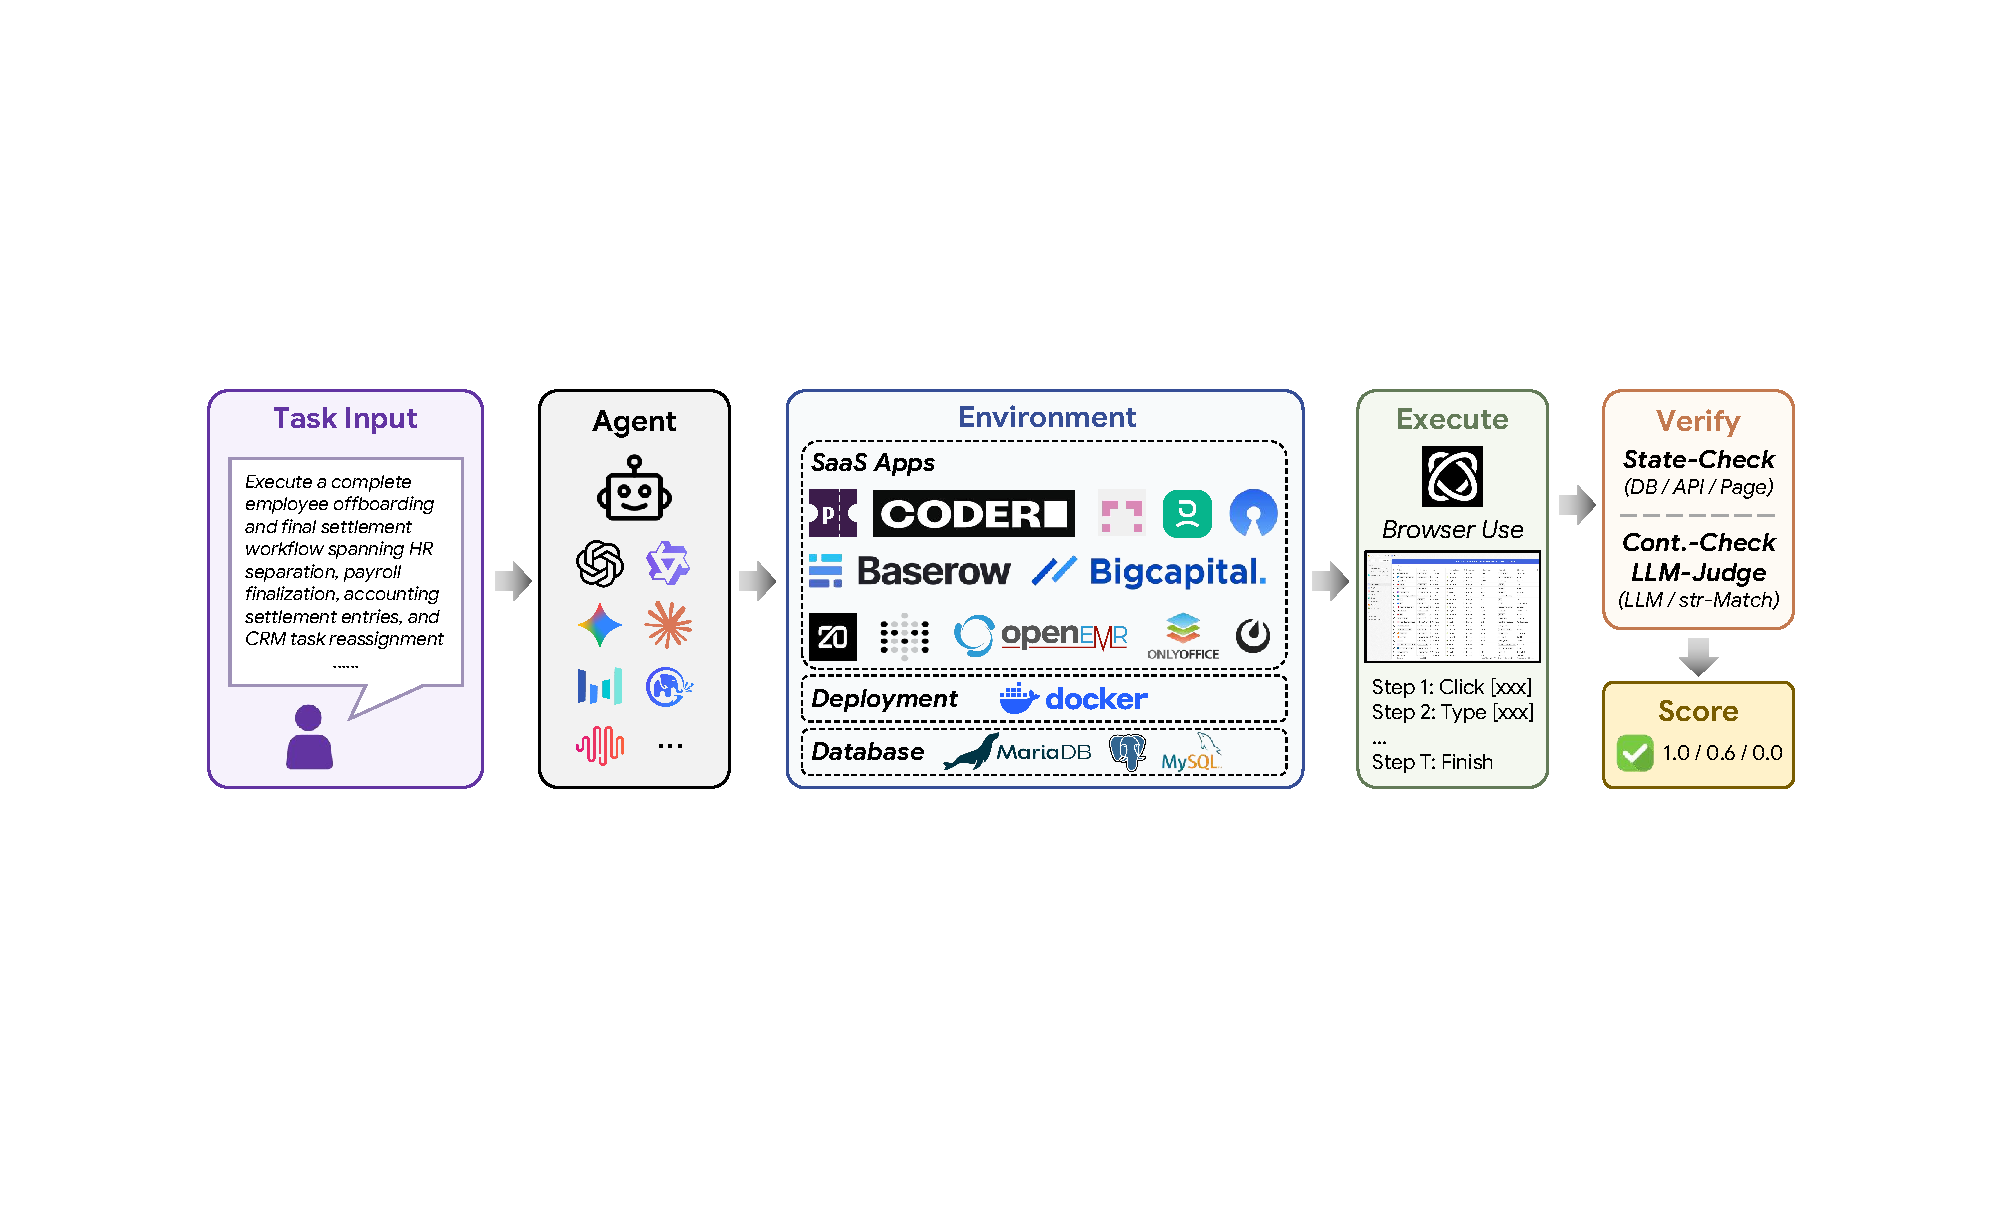
\includegraphics[width=0.86\textwidth]{fig/eval.pdf}
  \caption{\textbf{\datasetname 概览。}智能体接收自然语言任务指令，通过 browser-use 与本地部署的 SaaS 应用交互。执行结束后，验证工具评估任务结果，并汇总得到完全解决分数与检查点分数。}
  \label{fig:eval}
\end{figure*}

\begin{figure*}[t]
  \centering
  \begin{subfigure}[b]{0.50\textwidth}
    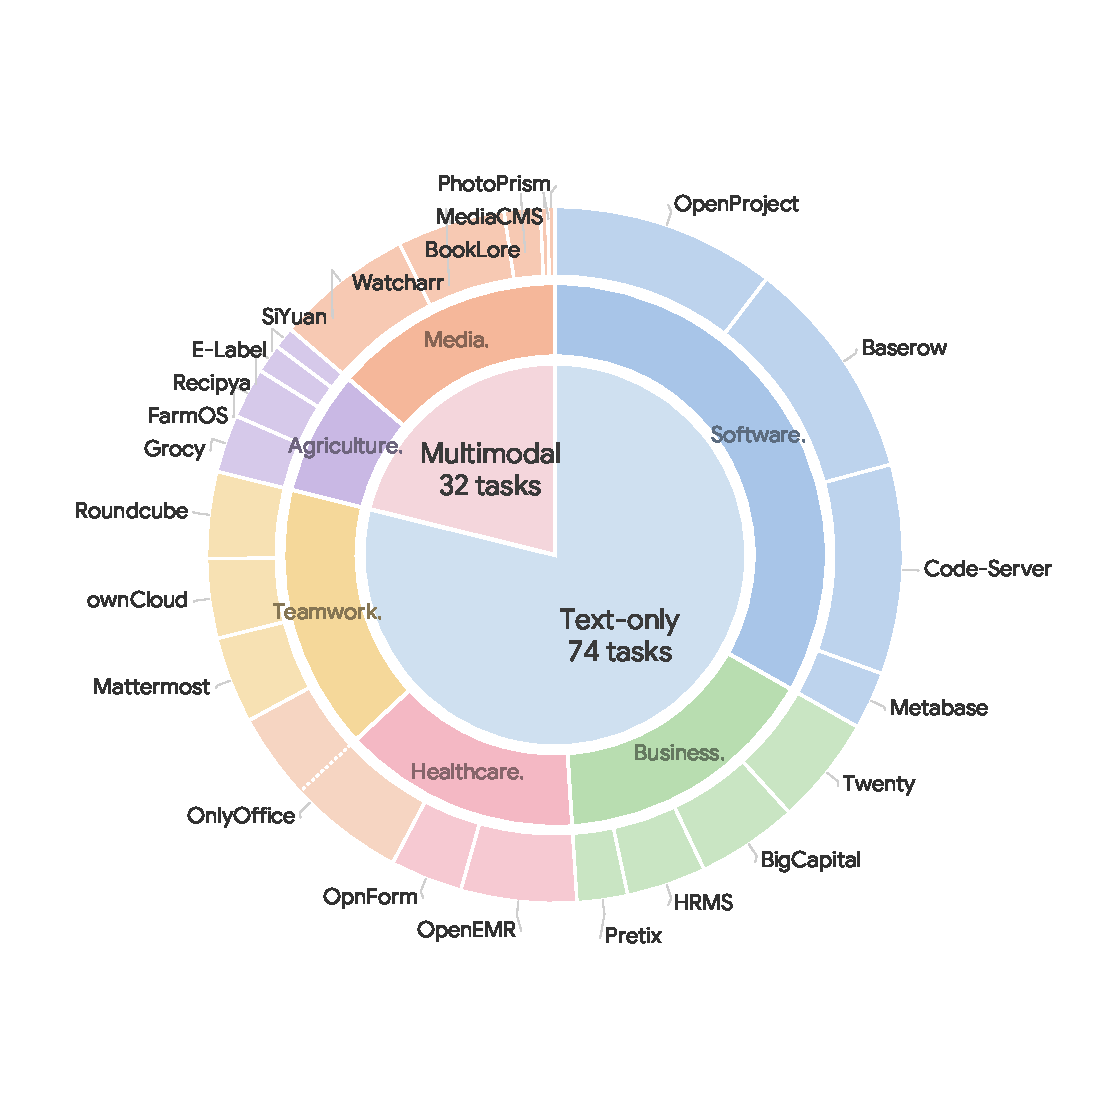
\includegraphics[width=\linewidth]{fig/panel_a_nested_donut.pdf}
    \caption{嵌套任务构成}
    \label{fig:stats-a}
  \end{subfigure}\hfill
  \begin{subfigure}[b]{0.45\textwidth}
    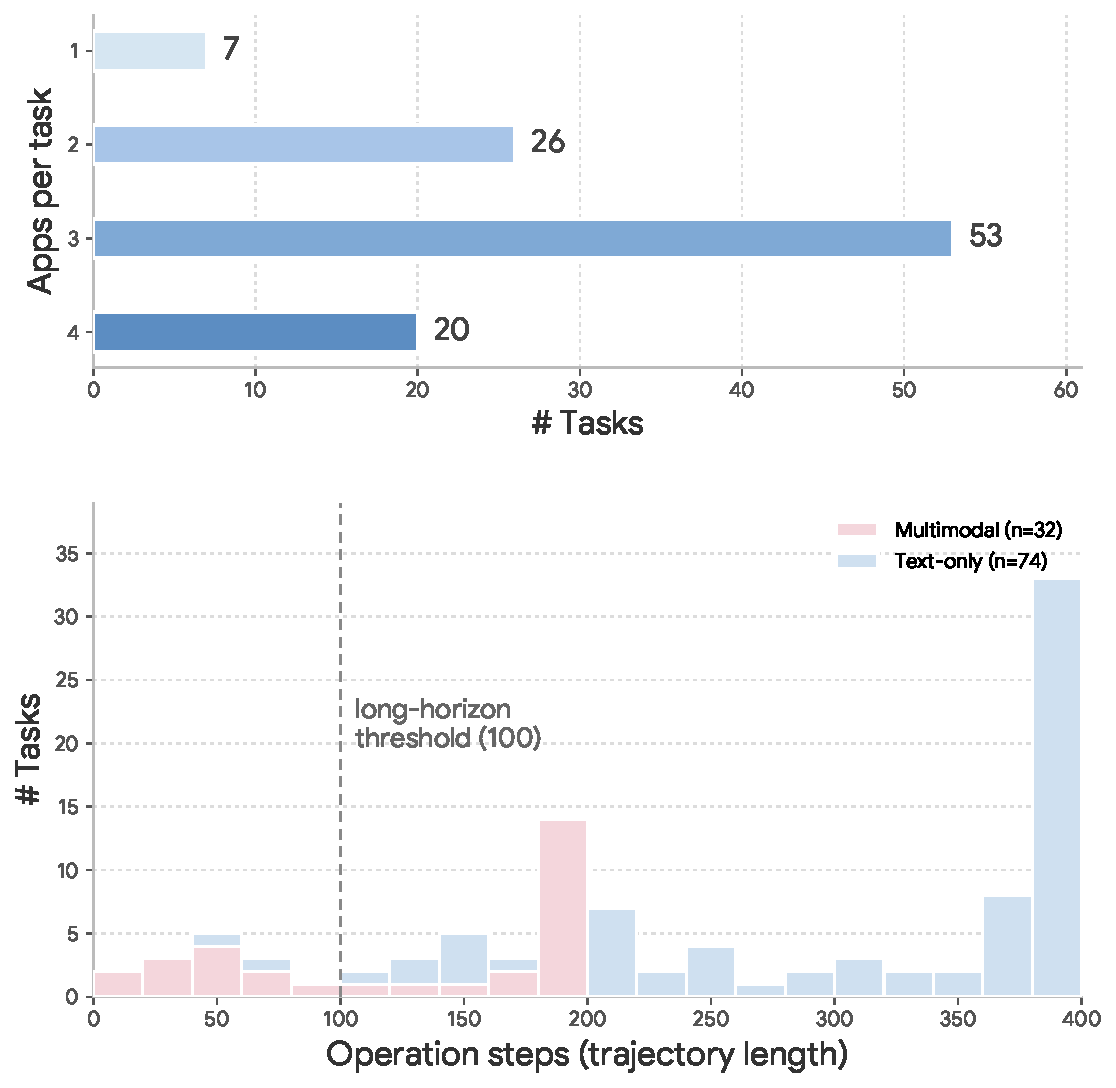
\includegraphics[width=\linewidth]{fig/panel_bc_combined.pdf}
    \caption{每任务应用数与任务跨度}
    \label{fig:stats-b}
  \end{subfigure}
  \caption{\textbf{\datasetname 的任务统计。}\textbf{(a)} 嵌套环形图展示任务在两种评测模态（纯文本与多模态）、六个领域及底层 SaaS 应用之间的构成；外环量化每个应用被使用的频率，体现基准所覆盖真实工具的多样性。\textbf{(b)} 上图给出每个任务涉及的应用数量，下图给出按模态堆叠的轨迹长度分布。两者分别从跨应用范围和操作跨度刻画任务复杂度。}
  \label{fig:task-stat}
\end{figure*}

\subsection{任务统计与设计}
\label{saas-task}

\paragraph{统计。} \datasetname 包含 106 个任务，横跨 23 个 SaaS 系统和 6 个专业领域。如图~\ref{fig:task-stat} 所示，我们从三个维度概括该基准：模态、领域与应用三个层次的嵌套任务构成；每项任务涉及的应用数量；以及根据 Claude Opus 4.6 执行轨迹估算的操作长度分布。基准包括 74 个纯文本任务和 32 个多模态任务；多模态任务主要集中在 Agriculture. 与 Media.，因为这些领域的工作流天然依赖图像、文档或媒体资产。\datasetname 具有很强的跨应用特征：106 个任务中有 99 个（93.4\%）至少涉及两个应用，三应用任务数量最多（53 个，占 50.0\%）。操作长度分布进一步凸显其长程属性：以 100 步为界，74 个纯文本任务中有 72 个（97.3\%）、32 个多模态任务中有 19 个（61.3\%）超过这一阈值。这些统计表明，\datasetname 强调需要跨应用协调和长程执行的真实专业工作流，而非孤立、短促的网页交互。

这些任务属性并非通过随机抽取应用功能获得。我们采用四阶段流水线：从专业角色和工作流种子出发，逐步合成、实例化并验证可执行任务。如图~\ref{fig:cons} 所示，该流程确保最终任务具备专业性、跨应用性、长程性和可验证性。

\paragraph{阶段 I：任务种子与角色定义。} \datasetname 的任务源自专业领域和面向工作流的设计原则。我们从上述六个领域出发，构建专业、真实且长程的任务。每个领域都实例化有代表性的职业角色，例如项目经理、财务运营人员、医疗行政人员、技术写作者、供应链协调员和媒体创作者。随后把这些角色的日常工作流抽象为任务种子，其中规定任务目标、领域语境、所需应用、预期证据、长程依赖和验证要求。

\paragraph{阶段 II：任务合成循环。} 给定任务种子后，我们使用由模板生成与任务实例化构成的两阶段迭代合成循环。每个阶段都由 LLM Builder 生成任务，再由人类专家 Challenger 和 Refiner 审查修订。LLM Builder 使用 Claude Opus 4.6。模板生成时，Builder 产生任务场景、目标、涉及的应用、跨应用依赖、参考步骤和预期结果；实例化时，它用应用入口、凭据、模式与数据状态、数据对象及多模态资产，把模板落地到具体环境。人类 Challenger 检查歧义性、完整性、可执行性与可验证性，包括多模态资产是否可访问、可读取且确有必要；人类 Refiner 随后接受或拒绝任务，或者附上修改意见退回。循环持续到任务被接受、拒绝或达到最大迭代次数。

\paragraph{阶段 III：静态检查。} 所有候选任务进入最终基准前都要经过专家质量控制。静态检查阶段根据任务描述、参考步骤、预期结果和验证逻辑进行评估，考察专业性、跨应用自然度、依赖深度、可验证性、叙事连贯性与复杂度质量，同时标记把 CRM 当作信息垃圾场、并行任务拼接和规格过载等常见反模式。

\paragraph{阶段 IV：执行检查。} 最后，专家亲自执行每项任务，并结合 \texttt{verify.py} 检查轨迹，重点考察任务与验证器是否一致、失败归因是否正确以及指令是否清晰。未通过静态检查或执行检查的任务会被修改或移除，只有同时通过两项检查的任务才纳入 \datasetname。

\begin{figure*}[t]
  \centering
  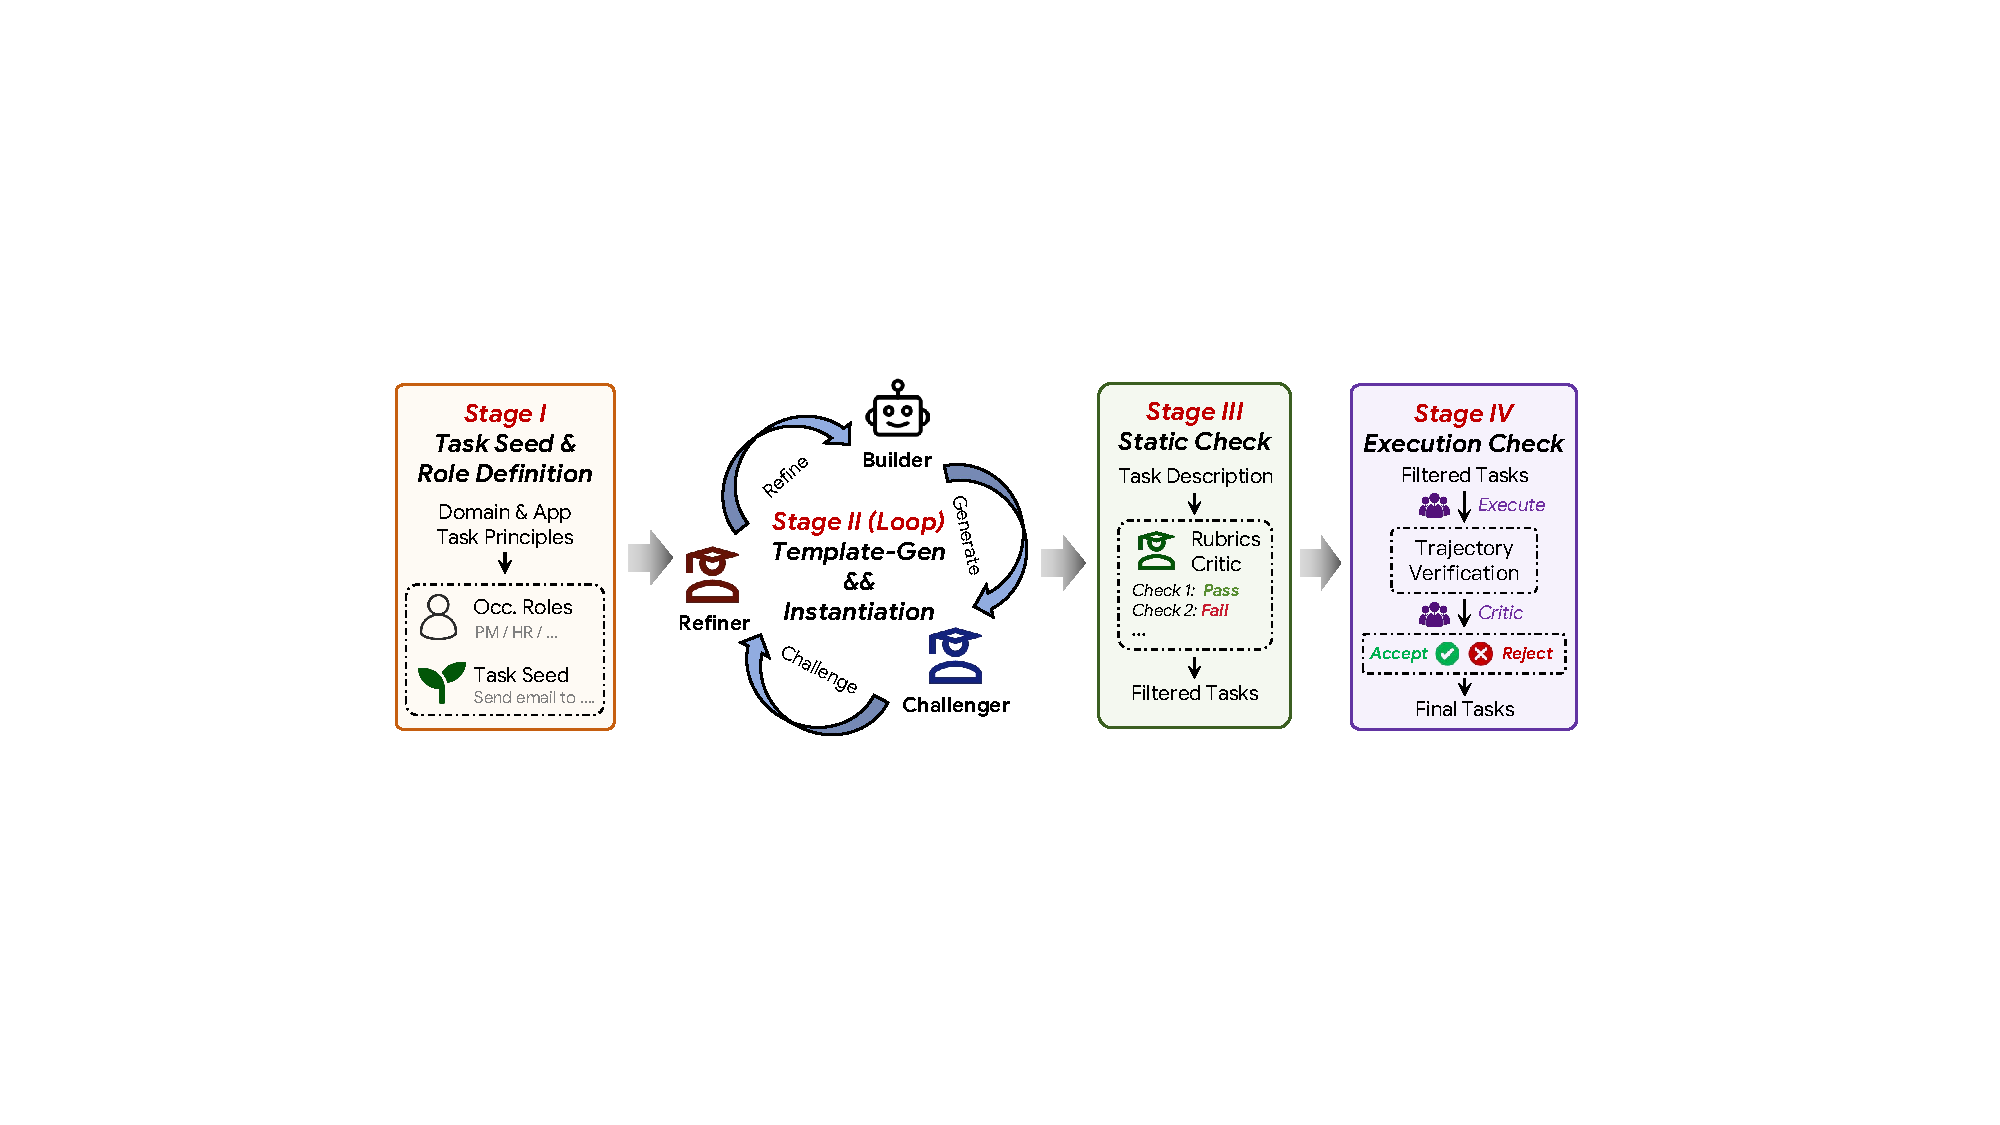
\includegraphics[width=0.9\textwidth]{fig/synthesis.pdf}
  \caption{\textbf{\datasetname 的任务合成流水线。}从特定领域的任务种子和职业角色出发，\datasetname 通过迭代的 Builder--Challenger--Refiner 循环生成模板并完成实例化；随后使用基于量规的静态检查和执行检查筛选生成任务，确保最终任务真实、可执行且可验证。}
  \label{fig:cons}
\end{figure*}

\subsection{评测协议}
\label{saas-eval}

所有待评智能体统一使用 browser-use~\cite{browseruse} 作为执行框架。每个智能体只能通过浏览器 UI 操作与 \datasetname 交互，包括导航、点击、输入和读取页面内容；不允许直接访问数据库、后端 API、文件系统或任务验证器。每项任务执行前，相应 SaaS 环境都会重置到预定初始状态，确保不同模型和不同运行之间能够公平比较。

每项任务被分解为一组验证检查点，每个检查点对应一个预期最终系统状态或任务产物，并分配相应权重。根据检查点性质，我们采用三类验证方法：\textbf{状态检查（State-Check）}，验证数据库记录、API 响应和文件是否存在等客观系统状态；\textbf{内容检查（Content-Check）}，通过结构规则和字符串匹配验证文档或文本输出；\textbf{LLM 裁判（LLM-Judge）}，评估无法可靠地用规则检查的开放式输出，例如报告质量或图像理解结果。补充材料提供了所有验证子类型的详细分类。检查点结果随后汇总，在严格任务层面和部分进展层面衡量成功情况。我们报告两项指标：
\begin{itemize}
  \item \textbf{完全解决分数（Resolved Score）}：仅当任务的全部检查点通过时取 1，否则取 0。
  \item \textbf{检查点分数（Checkpoint Score）}：根据通过的检查点计算带权部分分数，以反映长程任务中的部分进展。
\end{itemize}
